\section{Problem Formulation}
\label{sec:task}

We formally define the abstractive dialogue summarization
task with mathematical notations, and highlight the characteristics of this task by contrasting it with the well-studied document summarization
problem. Finally, we present a hierarchical classification of application scenarios, demonstrating the practicality of this task.

\subsection{Task Definition}\label{sec:taskdefinition}
A dialogue can be formalized as a sequence of $T$ chronologically ordered turns:
\begin{equation}
	D = \{U_1, U_2, ..., U_T\}
	\label{eq:dialogue}
\end{equation}
Each turn $U_t$ generally consists of a speaker/role $s_t$ and corresponding utterance $u_t = \{w_i^t|_{i=1}^{l_t}\}$. $w_i^t$ represents the $i$-th token\footnote{
%To construct input for neural models, tokenizers are used to convert text into tokens in the vocabulary
Texts are tokenized into tokens in the vocabulary as the input for neural models. Rare words may result in multiple tokens by algorithms such as Byte-Pair-Encoding. We do not strictly distinguish words and tokens in this survey.} in the $t$-th utterance, $l_t$ is the length of $u_t$.

Dialogue summarization aims at generating a short but informative 
summary $Y=\{y_1,y_2,...,y_n\}$ for $D$, where $n$ is 
the number of summary tokens. $Y$ and $\hat{Y}$ represent the reference summary and the generated summary respectively.



\subsection{Comparisons to Document Summarization}\label{sec:divergence}

Dialogue summarization is different from document summarization in various 
aspects, including language style and format, information density, 
discourse structure, and topic boundaries.

\begin{figure}[ht]
	\centering
	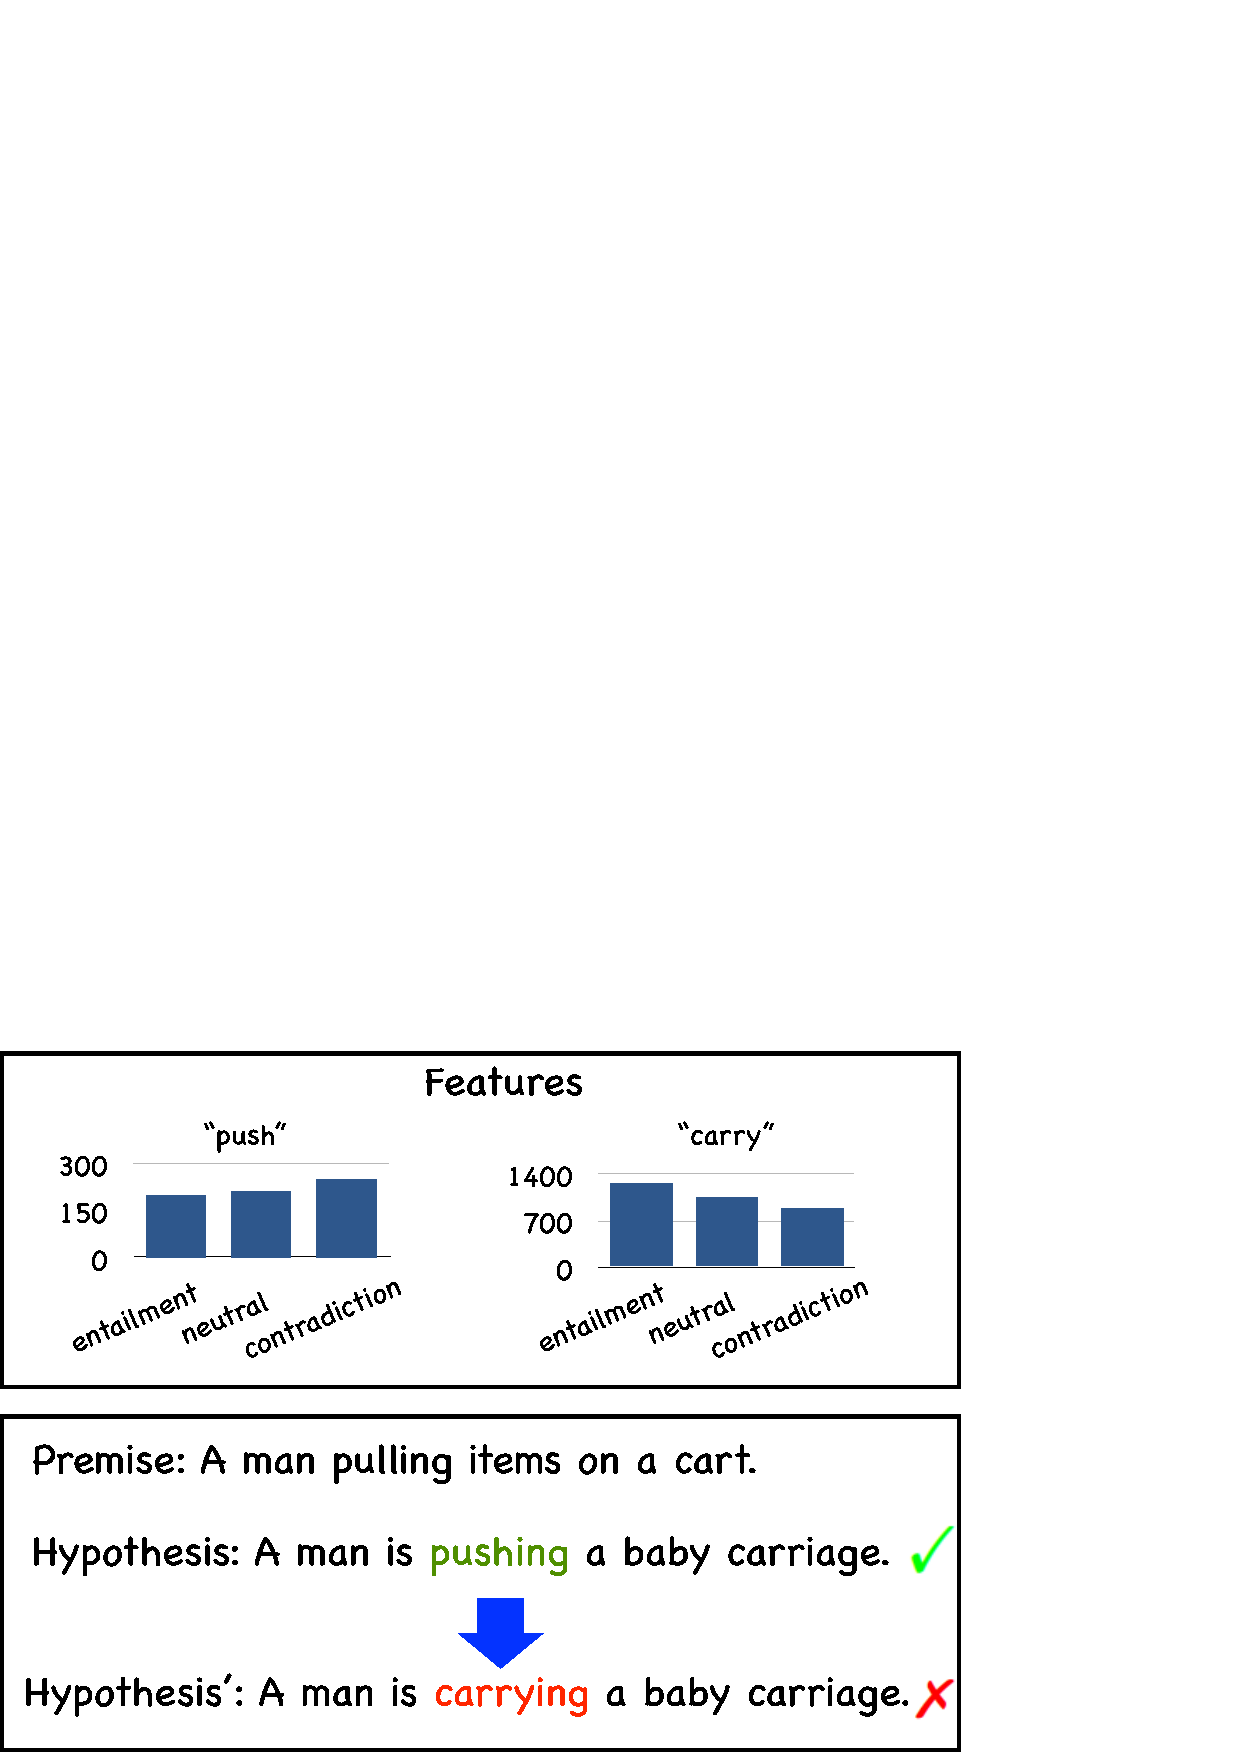
\includegraphics[scale=0.48]{fig/example.pdf}
	\caption{An example multi-party dialogue and its summary. The arrows represent unsequential dependencies between utterances. Elliptical sentences are in italic.}
	\label{fig:example}
\end{figure}

\textbf{Word Level - Language Style and Format:} 
Documents in previous well-researched summarization tasks are written from the third point of view, while dialogues consist of utterances expressed by different speakers in the first person. Informal and colloquial expressions are common especially for recorded dialogues from speech, such as ``Whoa'' in $U_6$ and ``u'' representing ``you'' in $U_7$ from Fig.~\ref{fig:example}.
Moreover, pronouns are frequently used to refer to events or persons mentioned in the dialogue history. Around 72\% of mentions in the conversation are {anaphoras} %pronouns
as stated in \citet{bai2021joint}. Meanwhile, the performance of coreference resolution models trained on normal text drops dramatically on dialogues~\cite{liu2021coreference}. All of these points manifest the existence of language style differences between documents and dialogues, posing a barrier in understanding the mappings between speakers and events in dialogues.


\textbf{Sentence/Utterance Level - Information Density:}
Document sentences are more self-contained with complete SVO (subject-verb-object) structures, while elliptical utterances are ubiquitous in dialogues, including $U_3$, $U_6$, $U_7$, $U_{11}$ and $U_{12}$.
Besides, the long dialogue can be summarized into a single summary sentence in Fig.~\ref{fig:example} as a result of back-and-forth questions and confirmations among speakers for communication purposes.
Question answerings, acknowledgments, and comments~\cite{asher2016discourse} are frequent discourse relations among utterances to narrow down speakers' information gaps and reach agreements.
In this way, dialogue utterances are highly content-dependent, and the information is scattered~\cite{zhang2021exploratory}, raising the difficulties for generating integral contents.

\textbf{Inter-sentence/utterance Level - Discourse structure:}
Articles tend to be well-structured, such as 
general-to-specific structure or deductive order. 
For example, the most important information 
in news summarization are always at the beginning of the document, resulting in a competitive performance of the simple Lead-$3$ baseline~\cite{see2017get}. However, it is not the same for dialogue summarization. Both Lead-$3$ and Longest-$3$, i.e. $\{U1, U2, U3\}$ and $\{U4, U8, U9\}$ in Fig.~\ref{fig:example}, get poor results in different dialogue scenarios~\cite{gliwa2019samsum,chen2021dialsumm,zhang2021emailsum}.
The dependencies among utterances are interleaved, shown by arrows in Fig.~\ref{fig:example}, and discourse relations in dialogues are more flexible,
even with the correction of wrong information. 
For example, 
Jake refused to be available for the reunion in $U_6$, but later agreed
in $U_8$.  As a result, it is more challenging to reason cross utterances for 
dialogue summarization than document summarization.

\textbf{Passage/Session Level - Topic boundaries:} Sentences under the same topic in documents are collected together in a paragraph or a section.
Previous works for extractive~\cite{xiao2019extractive} and abstractive summarization~\cite{cohan2018discourse} both took advantage of such features and made great progress. 
However, a dialogue is a stream of continuous 
utterances without boundaries, even for hours of discussion. The same topic may be discussed repeatedly 
with redundancies and new information, setting up obstacles for content 
selection in dialogue summarization.

%\JQ{it will be good to see the advantages of abstractive vs extractive approaches for dialogue summarization.}
%\JQ{add a little more about extractive methods, and explain why abstractive is more preferred especially in the case of dialogues.}
To better explain why abstractive approaches are more preferred than extractive ones, we list the result of the best rule-based extractive baseline, i.e., Longest-$3$~\cite{gliwa2019samsum}, the oracle extractive result determined by Rouge-L Recall score between each summary sentence and dialogue utterances~\cite{chen2018fast}, and the generation by BART fine-tuned on SAMSum dataset~\cite{gliwa2019samsum} of the dialogue in Fig.~\ref{fig:example} as follows:
\\
{
\scriptsize
\begin{tabular}{|p{1.5cm}|p{\linewidth-2.3cm}|}
	\hline
	\textbf{Longest-$3$} & Jessica: If I move some things around, I can too! Jake: Hell yeah man! You know I freelance, worst case scenario I'll work from wherever we are Jessica: We should meet up where we did last time, it's perfect middle for everyone.\\
	\hline
	\textbf{Oracle} & Jake: Hell yeah man! You know I freelance, worst case scenario I'll work from wherever we are\\
	\hline
	\textbf{BART}& Ted, Pia, Jessica and Jake are going to meet up on Friday night. \\
	\hline
\end{tabular}
}
\\
We can see that the readability of generated summaries are poor for Longest-$3$ and Oracle due to the language style and format difference. The compression ratio of Longest-$3$ is apparently low while it still misses the involvement of Ted and Pia as a result of low information density of dialogues. Oracle is concise but much more information is missing. The fine-tuned BART as an abstractive approach shows the favorable performance. 
%Therefore, abstractive approaches becomes the mainstream in researches on dialogue summarization. 
In a word, dialogue summarization is a valuable research direction, where the modeling and understanding of dialogues are challenging compared with document summarization and abstractive approaches are especially preferred.


\subsection{Scenarios for Dialogue Summarization}\label{sec:scenarios}

Considering the source of dialogues and the purpose of doing summarization,
we divide the application scenarios into two classes: \textbf{open-domain dialogue summarization (ODS)} and \textbf{task-oriented dialogue summarization (TDS)}. This taxonomy is similar to the one of dialogue systems~\cite{chen2017survey}. 
However, one should note that a pre-defined domain ontology is 
not necessarily required for TDS, which is different from that in 
task-oriented dialogue systems.
The application scenarios investigated in previous papers 
are classified into these two classes as shown in Fig.~\ref{fig:scenario}.

Open-domain dialogue summarization is further divided into daily chat, 
drama conversation, and debate \& comment. 
\textbf{Daily chat}~\cite{gliwa2019samsum,chen2021dialsumm} refers to the dialogues happening in our daily lives, 
such as making appointments, discussions between friends, etc. 
\textbf{Drama conversation}~\cite{rameshkumar2020storytelling,zhu2021mediasum,malykh2020sumtitles,chen2021summscreen} represents dialogues from soap operas, 
movies or TV shows, which are dramatized or fabricated with drama scripts 
behind them. Dialogues in these two classes are full of person names 
and events, resulting in narrative summaries about ``who did what''.
\textbf{Debate \& comment}~\cite{misra2015using,fabbri2021convosumm,chowdhury2019cqasumm} focuses more on question answering and 
discussions in online forums and arguments. These dialogues emphasize opinions or solutions to the given subject or questions.

Task-oriented dialogue summarization arises from application scenarios of different domains, which includes but is not limited to customer service, 
law, medical care and official issue.
\textbf{Customer service}~\cite{zou2021topic,feigenblat-etal-2021-tweetsumm-dialog,zhao2021todsum,liu2019automatic,chen2020jddc} refers to conversations between customers and service providers.
Customers start the conversation with their specific intents and agents are required to meet these requirements with the help of their in-domain databases, such as hotel reservations and express information consultation for online shopping. Dialogue summarization for this task is mainly to help service providers quickly go through solutions to users' questions for agent training and service evaluation. 
\textbf{Law}~\cite{fuzw20,duan2019legal,xi2020global} is dialogues related to legal service and 
criminal investigations. Dialogue summarization in this scenario alleviates the recording and summarizing workload 
for law enforcement or legal professionals. 
\textbf{Medical care}~\cite{joshi2020dr,song2020summarizing,song2020summarizing,zhang2021leveraging,liu2019topic} is dialogues between doctors and patients and medical dialogue summarization has some similarity to the research on electronic health records (EHR). Unlike the previous work focusing on mining useful information from EHR~\cite{yadav2018mining}, summarization is to extract useful information from the doctor-patient dialogue and generate an EHR-like or fluent summary for clinical decision-making or online search. It also aims to reduce the burden of domain experts.
\textbf{Official affair}~\cite{carletta2005ami,janin2003icsi,ulrich2008publicly,zhang2021emailsum} is conversations between colleagues for technical or teachers and students for academic issue discussion. They can be in the format of meetings or e-mails, with summaries covering problems, solutions, and plans.


\begin{figure}
	\centering
	\includegraphics[scale=0.65]{fig/scenarios.pdf}
	\caption{The classification of dialogue summarization tasks with different application scenarios. Datasets proposed for evaluations under each scenario are in \secref{sec:dataset}.}
	\label{fig:scenario}
\end{figure}


We compare and contrast ODS and TDS as follows.
\begin{itemize}
% functional role playing
\item Dialogues happen between \textbf{two or more speakers} both in ODS and TDS, whereas the \textbf{interpersonal relationship} and \textbf{functional relationship} among speakers are different. Generally, speakers in ODS are friends, neighbors, lovers, family members, and so on. 
They are equal either in the aspect of interpersonal relationships or functional relationships. For example, one can raise a question or answer others' questions in online forums~\cite{fabbri2021convosumm}.
In TDS, speakers have different official roles acting for corresponding responsibilities. For example, plaintiff, defendant, witness and judge in court debates~\cite{duan2019legal}, project manager, marketing expert, user interface designer and industrial designer in official meetings~\cite{carletta2005ami} are corresponding roles.
Among different dialogues, roles are the same and can be played by different speakers and a speaker's role is always unchanged for a service platform.
In a word, TDS pays more attention to functional roles while ODS focuses on speakers.


% covering topics
\item Multiple \textbf{topics} may be covered in the same dialogue session.
Topics in ODS are more diverse than in TDS. The summarization models are expected to deal with unlimited open-domain topics such as chitchat, sales, education, and climate at the same time~\cite{chen2021dialsumm}. 
However, topics in TDS are more concentrated and need more expertise for understanding.
Dialogues in TDS either focus on a single domain with more fine-grained topics, such as medical dialogues of different specialties,
or several pre-defined domains, such as restaurant, hotel, and transformation reservation.
Domain knowledge is significant for summarization, and it is divergent across sub-domains. For instance, expertise and medical knowledge are required in doctor-patient dialogues for generating accurate medical concepts~\cite{joshi2020dr} while specific knowledge bases for internal medicine and primary care are not the same.

%  inherent structure
\item The input dialogue for both ODS and TDS is made up of \textbf{a stream of utterance} as defined in Equation~\ref{eq:dialogue}. However, 
the \textbf{structure} of these two types of dialogues are different.
Open-domain dialogues often happen casually and freely while dialogues in TDS may have some inherent working procedures or writing formats. 
For example, the program manager in meetings usually masters the meeting progress~\cite{zhu2020end} implicitly with words such as ``okay, what about ...'', and communications by e-mails consist of semi-structured format including subjects, receivers, senders, and contents~\cite{zhang2021emailsum}. 

% special intentions for summaries
\item \textbf{Focuses of summaries} are distinct. Summaries for ODS in recent research are more like condensed narrative paraphrasing. An example is a synopsis from the Fandom wiki
%\footnote{\url{criticalrole.fandom.com}} 
maintained by fans for the Critical Role transcripts
%~\footnote{\url{github.com/RevanthRameshkumar/CRD3}}
\cite{rameshkumar2020storytelling}, helping to quickly catch up with what is going on in the long and verbose dialogues. Differently, dialogues in TDS take place with strong intentions for solving problems. Summaries for such dialogues are expected to cover the user intents and corresponding solutions, such as medical summaries for clinical decision making~\cite{joshi2020dr} and customer service summaries for ticket booking~\cite{zhao2021todsum}.%As a result, generating faithful content is extremely significant for TDS. %{faithfulness}
\end{itemize}

%\KZ{I feel that just dividing the dialogue summarization into ODS and TDS is a bit
%too coarse-grained. Later when you discuss the approaches, u need to associate
%each approaches with a certain characteristic/scenario of the task. It's more
%useful if u can use some refined characteristics of the task.}
